\documentclass{../beamer_template/myBeamer}


\DeclareMathOperator{\Cov}{Cov}
\DeclareMathOperator{\Var}{Var}
\DeclareMathOperator{\E}{\mathbb{E}}
\DeclareMathOperator{\Proba}{\mathbb{P}}

\newcommand{\Covb}[2]{\ensuremath{\Cov\!\left[#1,#2\right]}}
\newcommand{\Eb}[1]{\ensuremath{\E\!\left[#1\right]}}
\newcommand{\Pb}[1]{\ensuremath{\Proba\!\left[#1\right]}}
\newcommand{\Varb}[1]{\ensuremath{\Var\!\left[#1\right]}}

% norm
%\newcommand{\norm}[1]{\| #1 \|}

\newcommand{\indep}{\rotatebox[origin=c]{90}{$\models$}}





\usepackage{mathptmx,amsmath,amssymb,graphicx,bibentry,bbm,babel,ragged2e}

\makeatletter


\renewcommand{\addlogo}{
	\hfill	
	
\includegraphics[height=.4cm]{../beamer_template/figures/logos/iconOM.png}
	
\includegraphics[scale=1]{../beamer_template/figures/logos/openmole_dark.png}
}


\newcommand{\noun}[1]{\textsc{#1}}
\newcommand{\jitem}[1]{\item \begin{justify} #1 \end{justify} \vfill{}}
%\newcommand{\sframe}[2]{\frame{\frametitle{#1}\addlogo #2}}

\newenvironment{centercolumns}{\begin{columns}[c]}{\end{columns}}
%\newenvironment{jitem}{\begin{justify}\begin{itemize}}{\end{itemize}\end{justify}}

%\usetheme{Warsaw}
%\setbeamertemplate{footline}[text line]{}
%\setbeamersize{text margin left=15pt,text margin right=15pt}
%\setbeamertemplate{headline}{}
%\setbeamertemplate{footline}[frame number]
%\setbeamertemplate{navigation symbols}{}

\usetheme{Darmstadt}
\setbeamertemplate{headline}{}
\setbeamertemplate{navigation symbols}{}
\setbeamercolor{palette quaternary}{fg=primaryDarkOM, bg=primaryGreenOM}


%\setbeamercovered{transparent}
%\setbeamercolor{structure}{fg=purple!50!blue, bg=purple!50!blue}

\@ifundefined{showcaptionsetup}{}{%
 \PassOptionsToPackage{caption=false}{subfig}}
\usepackage{subfig}

\usepackage[utf8]{inputenc}
%\usepackage[T1]{fontenc}


\usepackage{tikz}

\usepackage{multirow}

\usepackage{mdframed}

%\usepackage[usenames,dvipsnames]{pstricks}
%\usepackage{auto-pst-pdf}


%\usepackage[dvipsnames]{xcolor}

\usepackage{threeparttable}


\usepackage{listings}
\lstset{language=Java} 

\makeatother



\title[DOE/Sensitivity Analysis]{Design of Experiments and Sensitivity analysis}
\subtitle{Course and practical application}
%\author[Short Author]{Author}
\author{ExModelo Summer School}
\date{June 24, 2019}
\institute{
\includegraphics[scale=2]{../beamer_template/figures/logos/openmole.png}}

\begin{document}



\begin{frame}[plain]
	\titlepage
\end{frame}
\addtocounter{framenumber}{-1}

\AtBeginSection[]
{
	\frame{
		\tableofcontents[currentsection, hideallsubsections]
	}
	\addtocounter{framenumber}{-1}
}




%\section{Introduction}


\sframe{Design of Experiments}{
\justify

\begin{itemize}
	\item Interactive model exploration by hand and the need for preliminary experiments
    \item The Design of Experiments (DOE) as the definition of computational experiments to extract information from the simulation model
    \item Example: NetLogo behavior space: basic grid DOE
    \item Sensitivity analysis as an advanced DOE
\end{itemize}

\bigskip

\textbf{Remark 1:} \textit{terminology strongly depends on disciplines and practices}

\medskip

\textbf{Remark 2:} \textit{most are generally \textbf{preliminary experiments} to prepare more elaborated, question-related, experiments}


}



\sframe{Outline}{
\tableofcontents
}


\section{Basic experiments}


\sframe{Basic experiments}{

\justify

\textit{Provide explicitly sampling points on which the model (or its replication task) will be run: notion of \textbf{direct sampling} in OpenMOLE (corresponds to DOE in the literature)}

\bigskip

\begin{itemize}
	\item full samplings
    \item elaborated sampling for high dimensions given a low computational budget (\textbf{the curse of dimensionality})
\end{itemize}

}


\sframe{One factor at a time}{
  
  
\justify  
  
Cheapest and intuitive DOE: \textit{all factors have nominal values and a discrete variation set, in which each is varied while others remaining fixed}

\bigskip

\begin{itemize}
  \item when model is slow - or computational budget highly limited
  \item does not capture interaction between parameters, and highly dependent on nominal values
  \item seen as a bad practice \textbf{BUT} useful for models taking significant time, and prone to thematic interpretation
\end{itemize}

  
}

\sframe{Example where One-At-a-Time fails}{

 %<img width=600 src=https://miniocodimd.openmole.org:443/codimd/uploads/upload_82c20b2e74a3f5b96a0fc227311cd516.png/>
 
 \centering
 
 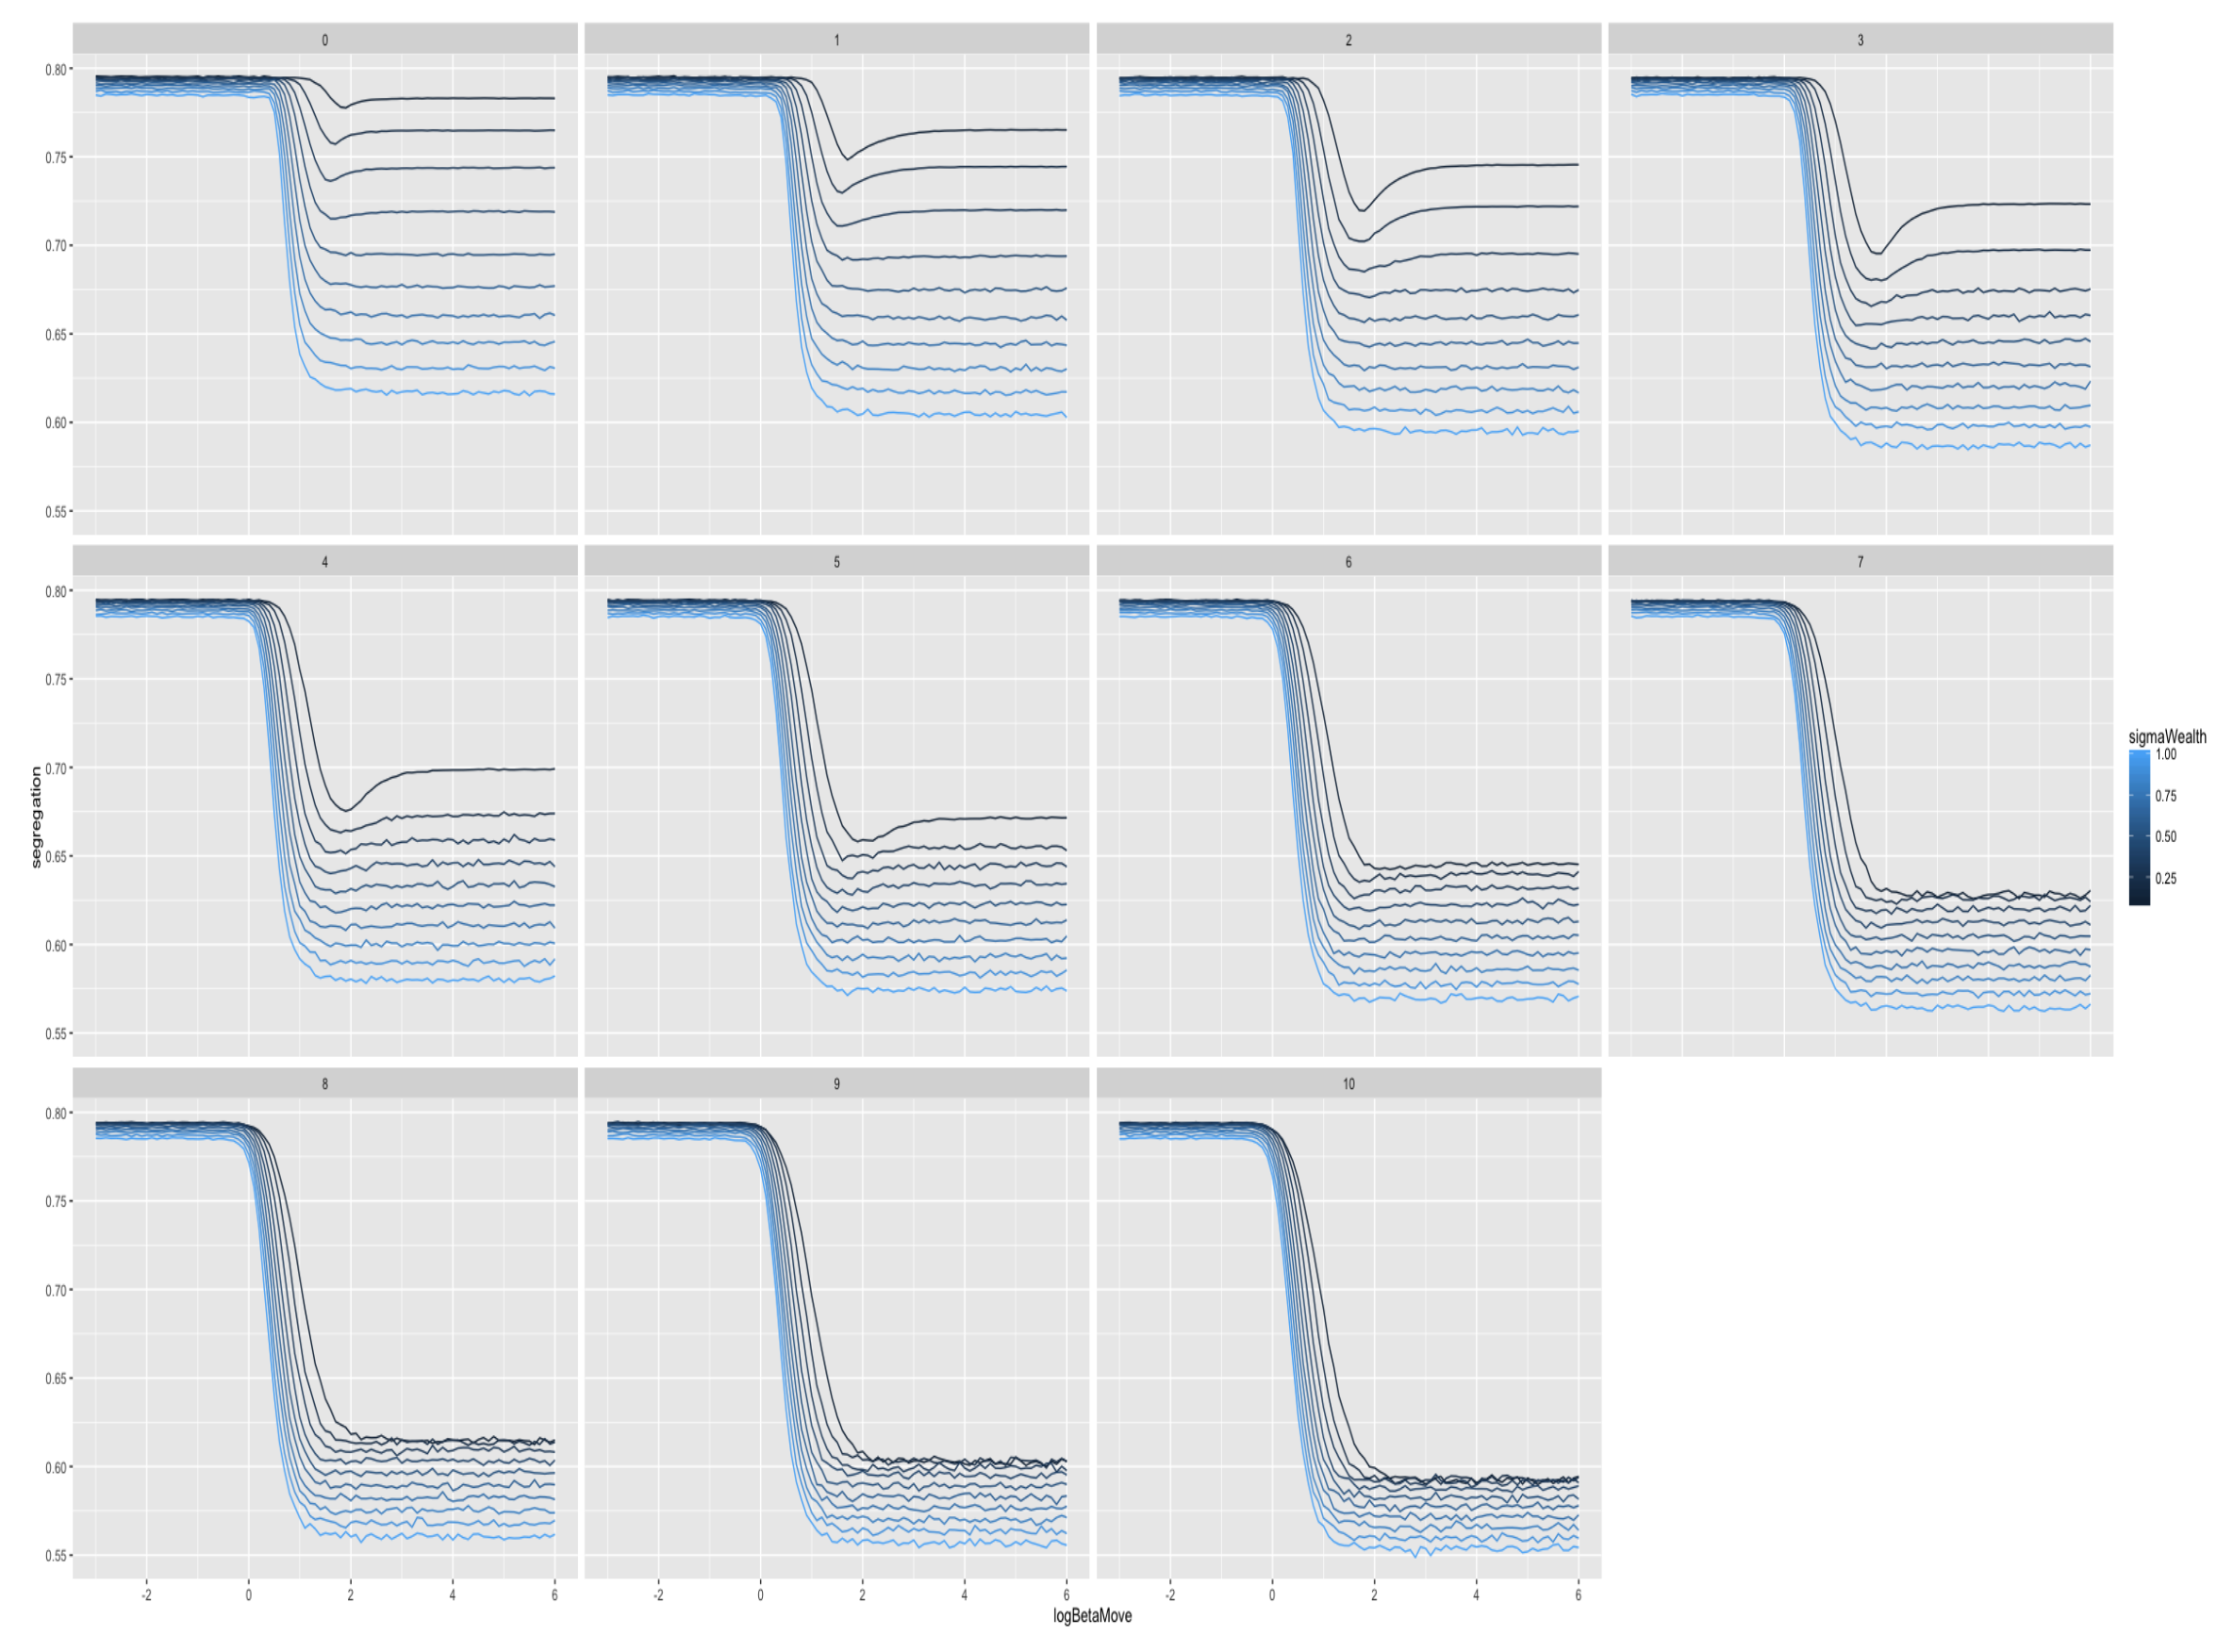
\includegraphics[width=\textwidth]{figures/example_oatfailure.png}
 
 

}


\sframe{Grid sampling}{



Brute force DOE: \textit{ensemble product of discrete variation ranges for factors (usually a regular grid but not necessarily)}

\bigskip


\begin{itemize}
  \item quickly limited by the curse of dimensionality - in practice still powerful with a quick model and a low number of parameters
  \item naive approach, i.e. only DOE for many "simulation-newcomers" such as economics or some parts of physics
\end{itemize}


}


\section{High-dimensional samplings}


\sframe{High-dimensional samplings}{

\justify

\textit{Computational limitations} $\implies$ \textit{need specific methods to efficiently sample the parameter space}

\bigskip

Different methods for improving sampling in numerical experiments given limited computational resources have been proposed, as for example:

\medskip

\begin{itemize}
	\item Sobol sequences (quicker convergence of integral estimation)
	\item Latin Hypercube Sampling
	\item Orthogonal sampling
\end{itemize}


}


\sframe{Low discrepancy samplings}{

\textit{Minimizing discrepancy for a point cloud: intuitively being spread evenly across the definition space}

\bigskip

%(def of discrepancy)
% The discrepancy is defined as the $L2$-norm of local discrepancy which is for normalized data points $\mathbf{X}=(x_{ij})\in \left[0,1\right]^d$, a function of $\mathbf{t}\in \left[0,1\right]^d$ comparing the number of points falling in the corresponding hypercube with its volume, by $disc(\mathbf{t}) = \frac{1}{n}\sum_i \mathbbm{1}_{\prod_j x_{ij}<t_j} - \prod_j t_j$. It is a measure of how the point cloud covers the space.

L2-discrepancy given for normalized data points $\mathbf{X}=(x_{ij})\in \left[0,1\right]^d$ by

\[
\left\lVert \mathbf{t} \in \left[0,1\right]^d \mapsto \frac{1}{n}\sum_i \mathbbm{1}_{\prod_j x_{ij}<t_j} - \prod_j t_j \right\rVert_2
\]

}


\sframe{Latin Hypercube Sampling}{


%|x|||||
%|:--:|:--:|:--:|:--:|:--:|
%||x||||
%|||||x|
%||||x||
%|||x|||

\begin{center}
\begin{tabular}{|c|c|c|c|c|}
\hline
	x & & & & \\\hline
	 & x & & & \\\hline
	 & & & & x \\\hline
	 & & & x & \\\hline
	 & & x & & \\\hline
\end{tabular}
\end{center}

\bigskip

\textit{Latin cube: one point in each row and column; hypercube generalization in any dimension}

}



\sframe{Sobol sequence}{

\textit{Sobol sequences are a case of quasi-random sequences with low discrepancy (also Halton sequences e.g.)}

\bigskip


\begin{itemize}
	\item Estimate integral in $1/N$ instead of $1/\sqrt{N}$ with random sampling
	\item Constructed recursively (using bit representations)
\end{itemize}

}

\sframe{Comparison of samplings}{

For $N=2500$ samples in 2 dimensions

\centering

\medskip

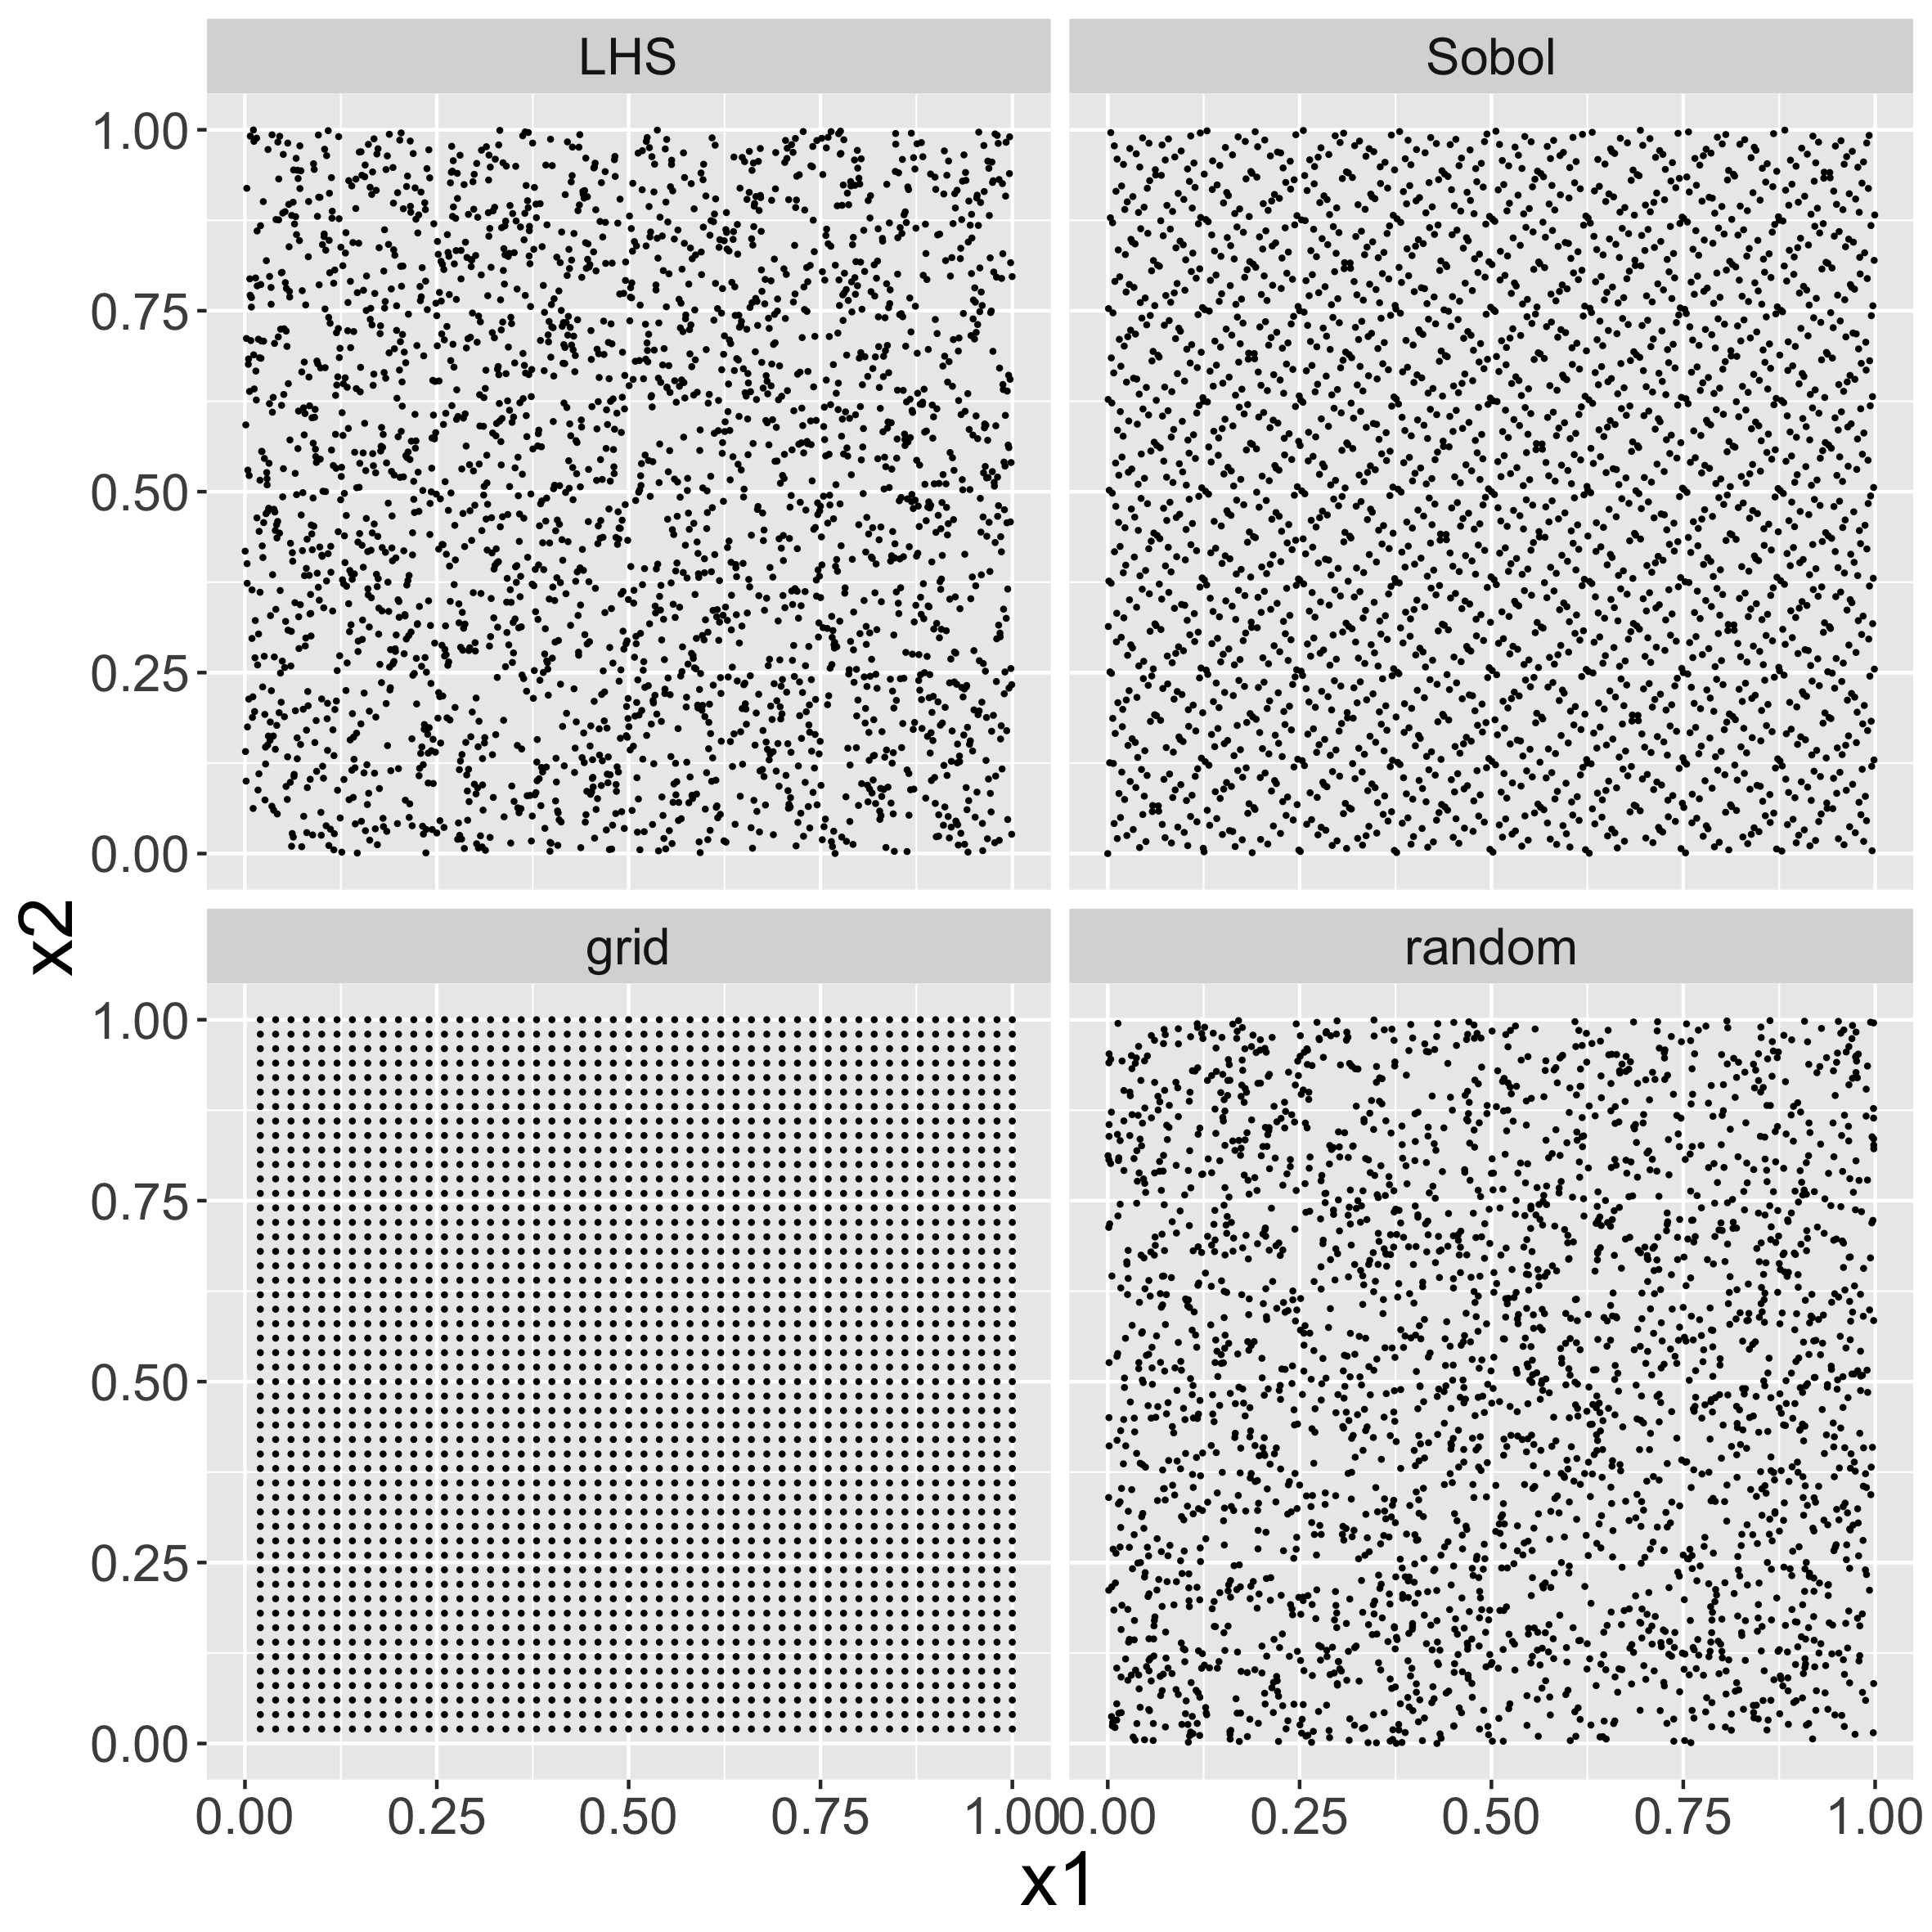
\includegraphics[height=0.8\textheight]{figures/sobol.png}

}



\section{Sensitivity analysis}


\sframe{Sensitivity analysis}{

\textbf{Aim of sensitivity analysis methods} \textit{How to summarize model sensitivity and isolate principal factors ?}

\bigskip


 \begin{itemize}
 	\item Most methods are \textit{global}, i.e. provide an aggregate of factor effect on the full parameter space
 	\item Advanced methods, still useful for preliminary experiments e.g. to discard factors from further experiments
 	\item Examples: Morris and Saltelli methods
 \end{itemize}



}


\sframe{Morris method}{

\justify

\textbf{Idea: } \textit{Sample trajectories in the parameter space in a One-At-a-Time manner. Screening method isolating \textbf{elementary effects}}

\bigskip

\begin{itemize}
  \item isolate local effects of factors
  \item more efficient than point sampling to get individual effects
  \item useful as a first experiment to understand the relative influence of factors
\end{itemize}

\bigskip

Introduced by \cite{morris1991factorial}, improved by \cite{saltelli2004sensitivity}, \cite{campolongo2011screening} propose to extend the method with Sobol sequences



}


\sframe{Saltelli method}{

Estimation of relative and conditional variances

\[
ST_i = \frac{E_{\mathbf{X}\sim i}\left[Var(Y | \mathbf{X}\sim i) \right]}{Var(Y)}
\]

}



\section{Application in OpenMOLE}


\sframe{OpenMOLE syntax}{

\textbf{Syntax of the direct sampling:}

\texttt{
val explo = DirectSampling(\\
 \hspace{1cm}evaluation = model,\\
 \hspace{1cm}sampling = \dots \\
)
}


}


\sframe{Example of samplings}{

  \textbf{One-factor sampling: }

\bigskip

\texttt{
 sampling = OneFactorSampling(\\
  \hspace{1cm}(x1 in (0.0 to 1.0 by 0.2)) nominal 0.5,\\
  \hspace{1cm}(x2 in (0.0 to 1.0 by 0.2)) nominal 0.5\\
 )
}

}



\sframe{Example of samplings}{

\begin{itemize}
 \item Grid sampling

\texttt{
sampling = \\
 \hspace{1cm} (x1 in (0.0 to 1.0 by 0.5)) x\\
 \hspace{1cm} (x2 in (0.0 to 1.0 by 0.5))
}
  \item LHS Sampling
  
\texttt{
sampling = LHS(\\
\hspace{1cm}100,\\
\hspace{1cm}x1 in (0.0,1.0),\\
\hspace{1cm}x2 in (0.0,1.0)\\
)
}

  \item Sobol sampling

\texttt{
sampling = SobolSampling(\\
\hspace{1cm} 100,
\hspace{1cm}x1 in (0.0,1.0),
\hspace{1cm}x2 in (0.0,1.0)
)
}

\end{itemize}

}


\sframe{Saltelli}{

\justify

\textit{Saltelli is a method in itself}

\bigskip

\texttt{
val sen = SensitivitySaltelli(\\
 \hspace{1cm} evaluation = (model on env by 1000),\\
 \hspace{1cm} samples = 100000,\\
 \hspace{1cm} inputs = Seq(\\
 \hspace{2cm} humanFollowProbability in (0.0,1.0),\\
 \hspace{2cm} humanInformedRatio in (0.0,1.0),\\
 \hspace{2cm} humanInformProbability in (0.0,1.0)),\\
 \hspace{1cm} outputs = Seq(totalZombified,halfZombified),\\
)
}
% TODO add hook


}



\sframe{Morris}{

\textit{Morris is also a method}

\bigskip

%\texttt{
%SensitivityMorris(
%    evaluation = modelExec on envLocal hook storeSimuCSV,
%    inputs = Seq(inputNumberOfCars in (1.0, 41.0), 
%                inputAcceleration in (0.0, 0.0099),
%                inputDeceleration in (0.0, 0.099)
%                ),
%    outputs = Seq(outputSpeedMin, outputSpeedMax),
%    repetitions = 100,
%    levels = 5)
%}

\texttt{
\noindent val morrisHook = \\
val sen = SensitivityMorris(\\
\hspace{1cm}evaluation = model on env hook morrisHook,\\
 \hspace{1cm} inputs = Seq(\\
 \hspace{2cm} humanFollowProbability in (0.0,1.0),\\
 \hspace{2cm} humanInformedRatio in (0.0,1.0),\\
 \hspace{2cm} humanInformProbability in (0.0,1.0)),\\
 \hspace{1cm} outputs = Seq(totalZombified,halfZombified),\\
 \hspace{1cm} repetitions = 100,\\
 \hspace{1cm}  levels = 5 \\
)
}



}



\section{Practical application}


\sframe{Practical application}{


Your turn to run some direct samplings and/or sensitivity analysis

\begin{itemize}
	\item given the described zombie model, what first experiment beyond stochasticity would be relevant ?
    \item write a script
    \item explore results (using e.g. the OpenMOLE GUI plots)
\end{itemize}

%\textit{Resources:}
% - one script running directsampling
% - example of grid explo results
% - example of Saltelli

}






%\backupbegin

%\appendix


%\sframe{Results of grid exploration}{

%\textit{Cooperation model}

%}




%%%%%%%%%%%%%%%%%%%%%
\begin{frame}[allowframebreaks]
\frametitle{References}
\bibliographystyle{apalike}
\bibliography{biblio}
\end{frame}
%%%%%%%%%%%%%%%%%%%%%%%%%%%%


%\backupend





\end{document}


